\documentclass[8pt]{beamer}
\usetheme{Goettingen}
\usecolortheme{dove}
\setbeamercovered{transparent}
\setbeamerfont{frametitle}{size=\normalsize} 
\setbeamertemplate{footline}[frame number]
\setbeamertemplate{itemize items}[circle]

\usepackage{mathrsfs} % equations
\usepackage{graphicx} % images
\usepackage[]{natbib} % citations + references
\bibliographystyle{unsrtnat} % citations + references


\title{Heat Kernel Smoothing}
\author[]{Gabriel Riegner}
\date{March 2025}

\begin{document}

% slide %
\begin{frame}{Heat Kernel Smoothing Using Laplace-Beltrami Eigenfunctions\\ \citep*{seo_heat_2010}}
\small
\begin{columns}
\column{0.5\textwidth}
\tableofcontents[hideallsubsections]
\column{0.5\textwidth}
\visible{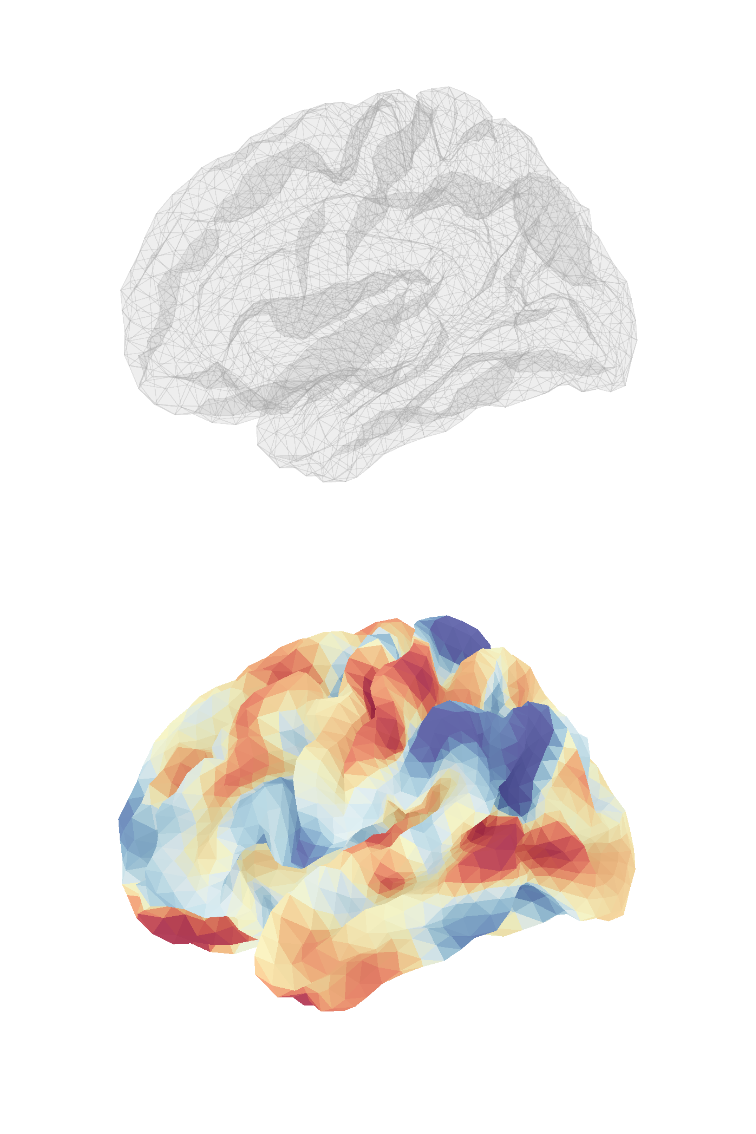
\includegraphics[width=0.8\textwidth]{project/figures/toc.png}}
\end{columns}
\vfill\centering
Gabriel Riegner, March 2025\\
DSC 291 Network Science and Graph Theory
\end{frame}

% section %
\section{Motivations}

% section %
\section{Paper Overview}
\begin{frame}{Definitions}
$Y$ defined on manifold $\mathcal{M} \subset \mathbb{R}^3$:
\begin{align}
    Y(p) = \theta(p) + \epsilon(p), \quad \epsilon(p) \overset{\text{iid}}{\sim} \mathcal{N}(0, \mathbb{I})
\end{align}

Eigenvalue problem for the Laplace-Beltrami operator $\Delta$ on $\mathcal{M}$:
\begin{align}
    \Delta \psi_j = -\lambda \psi_j
\end{align}

Heat kernel:
\begin{align}
    K_{\sigma}(p, q) = \sum_{j=0}^\infty e^{-\lambda_j\sigma} \psi_j(p) \psi_j(q)
\end{align}

Heat kernel smoothing:
\begin{align}
    K_{\sigma}  \ast Y(p) = \sum_{j=0}^\infty e^{-\lambda_j \sigma} \beta_j \psi_j(p)
\end{align}

\end{frame}

% section %
\section{Contributions}

% section %
\section{Simulations}

% section %
\section{Results}

% section %
\section{Conclusions}

% slide %
\begin{frame}{References}
    \small
    \bibliography{project/zotero}
\end{frame}

\end{document}